\documentclass[journal]{vgtc}                % final (journal style)
%\documentclass[review,journal]{vgtc}         % review (journal style)
%\documentclass[widereview]{vgtc}             % wide-spaced review
%\documentclass[preprint,journal]{vgtc}       % preprint (journal style)
%\documentclass[electronic,journal]{vgtc}     % electronic version, journal

%% Uncomment one of the lines above depending on where your paper is
%% in the conference process. ``review'' and ``widereview'' are for review
%% submission, ``preprint'' is for pre-publication, and the final version
%% doesn't use a specific qualifier. Further, ``electronic'' includes
%% hyperreferences for more convenient online viewing.

%% Please use one of the ``review'' options in combination with the
%% assigned online id (see below) ONLY if your paper uses a double blind
%% review process. Some conferences, like IEEE Vis and InfoVis, have NOT
%% in the past.

%% Please note that the use of figures other than the optional teaser is not permitted on the first page
%% of the journal version.  Figures should begin on the second page and be
%% in CMYK or Grey scale format, otherwise, colour shifting may occur
%% during the printing process.  Papers submitted with figures other than the optional teaser on the
%% first page will be refused.

%% These three lines bring in essential packages: ``mathptmx'' for Type 1
%% typefaces, ``graphicx'' for inclusion of EPS figures. and ``times''
%% for proper handling of the times font family.

\usepackage{mathptmx}
\usepackage{graphicx}
\usepackage{times}
\usepackage{epsfig}
\usepackage{epstopdf}
\usepackage[usenames,dvipsnames]{color}
%% We encourage the use of mathptmx for consistent usage of times font
%% throughout the proceedings. However, if you encounter conflicts
%% with other math-related packages, you may want to disable it.

%% If you are submitting a paper to a conference for review with a double
%% blind reviewing process, please replace the value ``0'' below with your
%% OnlineID. Otherwise, you may safely leave it at ``0''.
\onlineid{0}

%% declare the category of your paper, only shown in review mode
\vgtccategory{Research}

%% allow for this line if you want the electronic option to work properly
\vgtcinsertpkg

%% In preprint mode you may define your own headline.
%\preprinttext{To appear in an IEEE VGTC sponsored conference.}

%% Paper title.

\title{Parallel Topological Connection Reconstruction}

%% This is how authors are specified in the journal style

%% indicate IEEE Member or Student Member in form indicated below
\author{Robert Miller, Kenneth Moreland, Kwan-Liu Ma}
\authorfooter{
%% insert punctuation at end of each item
\item
 Robert Miller is a member of the ViDi group at the University of California, Davis. E-mail: bobmiller@ucdavis.edu
%\item
%#Utkarsh Ayachit works at Kitware, inc. E-mail: utkarsh.ayachit@kitware.com
\item
Kenneth Moreland works at Sandia National Laboratories. E-mail: kmorel@sandia.gov
\item
Kwan-Liu Ma leads the ViDi group at the University of California, Davis. E-mail: ma@cs.ucdavis.edu
}

%other entries to be set up for journal
\shortauthortitle{Miller \MakeLowercase{\textit{et al.}}: Parallel Topological Connection Reconstruction}
%\shortauthortitle{Firstauthor \MakeLowercase{\textit{et al.}}: Paper Title}

%% Abstract section.
\abstract{
 Many algorithms applied to mesh-based data structures are easily parallelizable because operations 
 can often be divided by the constituent elements of the mesh and 
 parallelized in large thread blocks.  The problem with this technique is 
 that when these threads generate new topological features, they tend to
 generate redundant information such as coincident vertices.  This 
 ``soup'' of elements requires significant additional memory to store the
 redundant information and fails to capture the adjacency of neighboring 
 elements.  We present a novel approach for the efficient construction 
 of connected topologies on massively parallel systems, which we demonstrate with 
 GPU and OpenMP implementations. In this approach, we use input
 topological features as a basis for efficient location of coincident
 features in the output.  We provide examples of the technique for 
 isosurface generation and multiple forms of tetrahedralization.
} % end of abstract

%% Keywords that describe your work. Will show as 'Index Terms' in journal
%% please capitalize first letter and insert punctuation after last keyword
\keywords{\textcolor{red}{TODO}}

%% ACM Computing Classification System (CCS). 
%% See <http://www.acm.org/class/1998/> for details.
%% The ``\CCScat'' command takes four arguments.

\CCScatlist{ % not used in journal version
 \CCScat{K.6.1}{Management of Computing and Information Systems}%
{Project and People Management}{Life Cycle};
 \CCScat{K.7.m}{The Computing Profession}{Miscellaneous}{Ethics}
}

%% Uncomment below to include a teaser figure.
%%\teaser{
%%\centering
%%\includegraphics[width=16cm]{CypressView.eps}
%%\caption{In the Clouds: Vancouver from Cypress Mountain}
%%}

%% Uncomment below to disable the manuscript note
%\renewcommand{\manuscriptnotetxt}{}

%% Copyright space is enabled by default as required by guidelines.
%% It is disabled by the 'review' option or via the following command:
% \nocopyrightspace

%%%%%%%%%%%%%%%%%%%%%%%%%%%%%%%%%%%%%%%%%%%%%%%%%%%%%%%%%%%%%%%%
%%%%%%%%%%%%%%%%%%%%%% START OF THE PAPER %%%%%%%%%%%%%%%%%%%%%%
%%%%%%%%%%%%%%%%%%%%%%%%%%%%%%%%%%%%%%%%%%%%%%%%%%%%%%%%%%%%%%%%%

\begin{document}

%% The ``\maketitle'' command must be the first command after the
%% ``\begin{document}'' command. It prepares and prints the title block.

%% the only exception to this rule is the \firstsection command
\firstsection{Introduction}

\maketitle

%% \section{Introduction} %for journal use above \firstsection{..} instead
Many existing parallel graphics techniques are designed to generate geometry from
some form of input mesh. Such algorithms tend to have the attribute that
computation of any given output feature depends solely on a small set
of input features. This provides a natural partitioning of the input
which can then be used to develop parallel algorithms. As an example,
the Marching Cubes \cite{Lorensen1987} algorithm can be parallelized per voxel, so that only
the data values at the voxel corners are necessary to generate the geometry
within the voxel (if any).

The problem with this naive parallelization is that it generates a
`soup' of output primitives, with no information about connectivity.
The aforementioned Marching Cubes algorithm simply produces a set of disconnected triangles.
This is not a concern so long as all further computation on the output
depends exclusively on the local attributes of individual primitives, such as is
the case with rendering. Rendering has often been the ultimate goal for the
generated output of parallel graphics algorithms and the size of the output is not a concern, so these techniques have been sufficient. When
additional processing of the output is desired that requires information about the connectivity 
between multiple primitives, the situation becomes more difficult. Consider the calculation of 
the curvature of the isosurface generated by Marching Cubes.
Given only a triangle soup, there is no simple method to determine the neighbors of any given triangle, which is a required step to 
compute the curvature. A more complex example would be the case of a visualization pipeline,
where different types of topological connectivity information may be necessary depending
on the structure of the pipeline.

This is not a new problem, and techniques exist to to determine topological
information about a primitive soup \cite{Park}. Generally this approach starts by finding 
and coalescing duplicate vertices, which may require a bounded radius nearest neighbor search to 
resolve vertices that are identical save for floating point error. Next, the algorithm finds all primitives that 
share two or more vertices, and links them together as neighbors. Finally,
some `duplicate' vertices may not actually represent desirable connections,
such as is the case where two cones meet at their apices, so these vertices
may need to be split in a final pass. This process is computationally complex, and is
specific to the topological connections between triangles. 

We would like to support a technique which applies equally well to other types of topological 
connections, such as determining the neighboring facets of tetrahedra. To this end, we have
explored the advantages of making a small modification to the algorithms that generate the
geometry, where information is stored about what feature of the input topology was used to generate
each output feature. For instance, Marching Cubes generates all output vertices on edges that
exist between the voxel coordinates of the input mesh.

To summarize, this paper is intended to make the following contributions:
\begin{itemize}
	\item{Provide a generalized technique for generation of topological connectivity information on highly parallel systems.}
	\item{Require no modifications to the algorithms generating geometry save for the
		storage of information about the input topological features used to generate each output feature.}

	\item{Make use of features of input topology to enhance the performance of the topology
		resolution technique.}

	\item{Demonstrate the effectiveness of our technique on the output of the Marching Cubes
		algorithm and a tetrahedralization algorithm.}
 
	\item{Show how knowledge of the output topology of an algorithm can be used to perform
		 simple mesh coarsening in the same pass as the topology resolution.}
 
\end{itemize}

We developed our technique for topology resolution so that it could be implemented
into the upcoming DAX framework, which will provide data analysis capabilities similar to those
in VTK, but targeted toward massively parallel architectures, beginning with the GPU.

\section{Previous Work}

We use Marching Cubes as an example of parallelized geometry 
generation \cite{Lorensen1987}. There are myriad existing isosurfacing implementations on the GPU, dating from 
Rottger's implementation \cite{Rottger2000}. Dyken provides a fairly 
detailed overview of the advancements in GPU implementations of Marching Cubes and 
Marching Tetrahedra \cite{Dyken2008} .

The basic topology resolution technique described in the introduction section is
introduced by Park et al. \cite{Park}. Additionally, Kipfer mentions
implementing a topology construction technique along with their GPU
Marching Cubes algorithm \cite{Kipfer2005}. Kipfer's technique involves the use of the edges that vertices 
will be placed on as a key for determining which vertices would be duplicated. Kipfer 
thus avoids the multiple computation of such vertices and avoids the need for coincident 
point resolution. To have accurate normals at the generated vertices, Kipfer's technique
requires precomputation of the gradient of the volume at the voxel vertices. Any other
interpolable attributes to be derived from the volume must also be precomputed at the
voxel vertices. Our method for determining dulateplicate vertices extends Kipfer's method in that
we may key off of any input feature.

Stream compaction is an important element for efficient geometry generation on the GPU.
Horn provides an early method for stream compaction on the GPU \cite{Horn2005}, which
was improved upon by Sengupta \cite{Sengupta2007}, who also provides a CUDA implementation. 
These approaches rely on the data parallelism technique and the application of prefix sums 
as described by Blelloch \cite{Blelloch1990}. Dyken further optimizes
GPU compaction techniques by making use of a data structure called a Histogram Pyramid \cite{Dyken2008}.
For our examples, we use geometry generation methods that make use of the prefix-sum
method of compaction, but other compaction techniques such as histogram pyramids could be
substituted for the prefix sum technique for increased performance in any case where our method is applied.

We use coincident point resolution (vertex welding) in Marching Cubes with the Thrust
C++ template library \cite{Bell2012}. Bell, a primary
developer of the Thrust library, also presents a vertex welding technique as an
example application of Thrust \cite{Bell2010}. Bell also notes that GPU sorting techniques can
be instrumental in the development of high-performance GPU algorithms. Hoberock uses a
lexicographic sort directly on the vertices generated by Marching Cubes, then collapses 
duplicates to get the final welded surface. Our approach has many similarities, but we
differ in the basis for the sort and in the method of collapsing duplicates. We
can apply the technique to arbitrary input topologies and also avoid invalid results when
floating point errors exist in the vertex coordinates.

Carr et al. \cite{Carr2006} describe several ways to subdivide voxel grids into tetrahedral grids. To fairly test performance of our topology generation on unstructured grids, we generate each of these subdivisions and demonstrate that the performance of our approach is similar in all cases.

Observant readers may notice a similarity between our proposed algorithms and those supported by the MapReduce framework \cite{MapReduce}. Like MapReduce, our algorithms first map keys to values then collect keys and reduce the values. Although we believe our algorithms could be implemented in a MapReduce framework (an exercise we leave to the reader), it would require additional collection operations to resolve topological connections. Other researchers 
\cite{Stuart2010}\cite{Vo2011} have implemented visualization algorithms directly in MapReduce, but they serve purposes other than those we address.

\section{Methods for Merging Algorithm}
Without significant modification of the algorithms generating topological features,
we present an approach that reconstructs the topological connections
between these features. By topological connections, we are referring to the information necessary to
determine all topological features that are adjacent to any individual feature of 
interest. We assume and provide a representation based on point arrays and either implicit or explicit cell connection lists. Generating incidence lists, such as the list of all cells incident to a point, is a trivial extension to our algorithm. Given a point P 
generated by the Marching Cubes algorithm, the topological connections
could be a list of all faces that contain point P as a vertex. Depending on
the intended use of the topology, it may be preferable to store the list of
points Q where there exists an edge (P,Q). Our approach can be applied
to generate any of these forms of connectivity information.

\subsection{Goals}
In developing our technique for reconstruction of topological connections, we have the
following requirements.
\begin{itemize}
	\item{Support at least the following feature types: vertices, edges, faces and facets.}

	\item{Require minimal modification to the algorithms used to generate topological features.}

	\item{Work as an efficient data-parallel method}
 
\end{itemize}

\subsection{Algorithm}
Our technique was developed by generalizing and extending the vertex welding example from the Thrust library \cite{Bell2012}.
Since many vertices are redundant when all triangles in a mesh are stored discretely, it is often desirable to
'weld' the duplicate vertices to single instances. We base our technique on the Thrust method because it has a similar
structure to the approach we take for topology generation, and because it is designed to work with nVidia CUDA platforms as well as platforms supported by OpenMP. The algorithm works as follows:
\begin{itemize}
	\item{Given an array of point coordinates $V_1$:}
	\begin{enumerate}
		\item{Lexicographically sort $V_1$ so that duplicate vertices are placed together in the array.}
		\item{Take the first element from each group of duplicates and store it in an output array $V_2$.}
		\item{Find the new index in $V_2$ for each vertex in $V_1$ and store it in an output array $Map_{1\rightarrow 2}$, which serves as a many-to-one mapping of points in $V_1$ to $V_2$.}
	\end{enumerate}
	\item{Return $V_2$ and $Map_{1\rightarrow 2}$ as output.}
\end{itemize}

The above algorithm is a good basis for an algorithm to generate topological connectivity because it allows for
grouping and processing of duplicate vertices. Since we can store which triangle generated each copy of a duplicate vertex,
 the above algorithm can be adapted to calculate a neighboring face list for each point. Therefore, using the Thrust
algorithm as a basis, we set out to create a technique that could be used for generating topological connectivity information 
from multiple kinds of disconnected input geometric elements. There are several requirements for this which the Thrust algorithm
does not immediately meet.

Unlike the creators of the Thrust algorithm, we are not interested specifically in the elimination of duplicate elements. Instead, we want
to form groups of geometric elements and then merge these into an output. These elements may not be simple vertices as in the Thrust example.
To use this for the generation of topological connections, we will need to associate attributes with each vertex. To this end, rather than taking as input an array of vertices,
we take in an array of geometric elements of some unspecified type. Often, the input will be an array of `tuples' which may consist of
vertices and their associated attributes such as normals or polygon IDs. Hereafter, we will refer to this input array as the `mergeable' array.

The Thrust algorithm groups bitwise-equal elements together. 
This would be inappropriate if additional attributes were associated with
each sample of a given vertex. For instance, three vertices at the same location that possess different normal vectors
would not compare bitwise equal, but we may wish to process them as a group. To resolve this, we take in an array of `keys' where
each key corresponds to an element of the mergeable array. The key for each mergeable element will be compared against the keys for
other mergeable elements using a user defined comparison operator $keycomp$. $keycomp$ is required to be analagous to the less-than operator, so
it takes two keys as input and must return $true$ if the first element should be placed earlier in the array than the second element, and $false$
otherwise. If $keycomp(k_1, k_2) = false$ and $keycomp(k_2, k_1) = false$, then the elements are assumed to be part of the same group and will be merged.

The keys can be based off of point coordinates as is done in the Thrust welding example. However, keys based on floating point numbers such as coordinates are inferior because of the large number of bits required to represent them and the high probability of small numerical errors leading to lexicographic differences. Later in this paper we present algorithms with more efficient keys.

Since we no longer require elements of each group to be bitwise
equal, we cannot simply use the first element of the group for our output vector. Instead, we will rely on two user-defined operators
which together will merge the grouped elements to a single output. The reason for having two operators is that some operations, such
as averaging, require two steps; in this case, the first operator would be a sum, and the second operator would be a divide. In our
implementation, we restrict the first operator, hereafter referred to as a merge, to be analagous to a sum: a binary operator that is commutative and associative. We restrict the input and output types of this operator so that it must take in two geometric elements and output a version that merges the elements' properties in some way.
Likewise, we restrict the second operator, hereafter referred to as a transform, to be analagous to scalar division: a binary operator taking one geometric element and the number of elements in the
group as input. The return type of the transformation operator is unrestricted, and the result of these transformations will be passed as the output of our algorithm. 

Finally, for this technique to be useful it must be possible to determine where each element of the mergeable array is mapped to in the output array. 
Our algorithm will therefore return an array of the new indices for each of the input elements.

With these modifications, we provide a generalized method to group various 
types of geometric elements and then merge each group into single outputs. A high-level overview of the algorithm follows:

\begin{itemize}
	\item{Given:}
	\begin{itemize}
		\item{An array of mergeable elements $M$}
		\item{An array of keys $K$ of the same size as $M$}
		\item{A key comparator $keycomp(k_1, k_2) \rightarrow bool$}
		\item{A merging operator $merge(m_1, m_2) \rightarrow m_3$}
		\item{A transformation operator $transform(m_1, GroupSize) \rightarrow Output$}
	\end{itemize}
	\begin{enumerate}
		\item{Sort $M$ using the key array $K$ and the key comparator $keycomp$ to divide $M$ into groups.}
		\item{Determine the new indices for each element and store them in an output array $Map_{1\rightarrow 2}$.}
		\item{Merge the elements of each group in $M$ into single elements using the $merge$ operator and store in an array of mergeables $N$. During this process, maintain a count of the number of elements merged to form each group, storing these in an array $C$}
		\item{Transform each element in $N$ into outputs using the $transform$ operator with the sizes from $C$ and store in an array of outputs $O$.}		
	\end{enumerate}
	\item{Return the output array $O$, the new index array $Map_{1\rightarrow 2}$, and the group sizes $C$ as output.}
\end{itemize}

To provide a more concrete example, our templated CUDA implementation of this technique using the Thrust library is available in the supplemental material.

\section{Methods for Mesh Generation}
In order to test our method for generation of topological connectivities on a range of data types, we made use of several techniques to generate geometry.
To test with data calculated along a structured grid, we used the Marching Cubes algorithm to generate contour surfaces from input volume data. Next, to test
with data from unstructured grids, we tetrahedralized the volume in each of the manners as presented by Carr, et al. \cite{Carr2006}. We generated contour surfaces from these tetrahedralizations
to get similar data as from the Marching Cubes results but from an unstructured grid. Additionally, we use the tetrahedralizations directly as the input to test our technique
to find the topological connections of a 3D structure.


\subsection{Performance Measurement}

We measure performance on a test system containing an Intel Core i7 975 Processor, which has a clock speed of 3.33GHz. Our test system has 12GB of RAM, and contains 2 nVidia Tesla C2070 cards. The datasets we use for testing are shown in Table~\ref{tab:datasets}. For all OpenMP tests, we set the number of threads to 8.


\begin{table}[h!]
\begin{center}
\begin{tabular}{p{2.7cm} p{1.9cm} r}
Name & Dimensions &  Tris (MC)\\
\hline
Spherical Distance A & 64x64x64 & 35,996\\
Spherical Distance B & 128x128x128 & 149,420 \\
Spherical Distance C & 256x256x256 & 607,388 \\
Spherical Distance D & 512x512x512 & 2,451,212 \\
MRI Head A& 64x64x64 & 138,510 \\
MRI Head B& 128x128x128 & 789,440 \\
MRI Head C& 256x256x256 & 4,947,294 \\
\end{tabular}
\end{center}
\caption{Test Datasets}
\label{tab:datasets}
\end{table}


The isovalues used for contour generation are consistent for all tests within each dataset, and are chosen to show relevant features of the dataset. We perform Marching Cubes, Marching Tetrahedra and several tetrahedralizations on each dataset to produce input geometry. All reported times in all tables are in milliseconds.  The Thrust library does not currently support spanning operations over multiple GPUs. We make use of two GPUs for our measurements by partitioning the input and performing the algorithm separately on each, then merging the results.


\subsection{Method of Topological Connectivity Construction}
Our technique is an extension of existing vertex welding methods. We will first analyze the original vertex welding approach and the manner in which we extended it for topological connectivity construction. We will then discuss methods of performance improvement of the original vertex welding method that we can achieve due to our extensions. Finally, we will discuss the usage of our extensions for the generation of topological connectivity information for various types of geometric inputs.

\subsubsection{Vertex Welding}

Because we made several modifications and extensions to the original vertex welding technique, we measure the additional performance
cost of our implementation of the technique as compared to the original. To perform a fair comparison, it is necessary to apply our technique to the same task. Vertex welding with
our generic group-merging algorithm can be accomplished by specifying the following inputs:

\begin{itemize}
\item{The array of mergeables $M$ should be an input array of vertices.}
\item{The array of keys $K$ should be the same array as $M$.}
\item{The key comparitor should compare vertices lexicographically.}
\item{The merge operator should return the first element.}
\item{The reduction operator should simply return the given element.}
\end{itemize}

For the purposes of vertex welding, we ignore the $C$ output of the group merging algorithm, and treat the outputs $O$ and $Map_{1\rightarrow 2}$ as the original algorithm's outputs $V_2$ and $Map_{1\rightarrow 2}$, respectively.

Although we were able to measure the performance differences using this technique, it provides no benefit over the original implementation. Also, our generated contour surfaces contain per-vertex normals and several scalar attributes, and this approach loses all information for these associated attributes except for the first instance of each vertex. To resolve this, we substitute a merge operator that sums these attributes, and a reduce operator that divides by the group count (and renormalizes the normal vector) so that our output vertices contain an averaged sample of the attributes from each merged instance. We then measure the performance impact from this change.

\label{sec:IntegralIDs}
To improve performance over the initial technique, we make use of our ability to use input keys other than the original vertices. Initially we considered the case of the output of our structured grid
approach, Marching Cubes. In this case, we know a good deal about the input topology on which the output is generated that was not previously being used to help generate the topological connections. Specifically, the output vertices from Marching Cubes are generated only on the edges of input voxels. Each of these edges is shared by at most four voxels (ignoring degenerate vertex intersections), so there can be at most four instances of any one vertex.
We assign each unique edge in the voxel grid an implicit integer ID, then store the corresponding edge ID for each vertex generated by Marching Cubes. Other than the additional storage requirement, this modification causes no measurable change in the performance of geometry generation, but significantly improves performance during vertex welding. Because it is known that these keys are identical if and only if the vertices are identical, we hypothesize that by using these integer IDs as the keys in the group-merging algorithm we noticeably improve the performance of the technique due to the simpler comparison operations for the sorts. 

We next consider the case of unstructured grid inputs. In this case edges cannot in general be implicitly assigned IDs, so they must be built from vertex IDs, which are implicit. We pair vertex IDs (least to greatest) to form a unique integral ID for each edge of the unstructured grid and store this as an attribute of the output vertex. 

Using the integer ID approach described above carries an additional advantage. From our Marching Cubes and Marching Tetrahedra implementations, we find that the Thrust approach often fails to weld meshes as expected. We trace this failure to the fact that some vertices that should be identical actually differ slightly due to floating point error, and thus are not bitwise equal as required by the Thrust approach. Such errors are exceptionally easy to encounter: since floating-point operations are not associative, our errors are generated simply by failing to ensure that we always use the same vertex order when generating interpolants. By assigning integral IDs to the output vertices, our approach is agnostic to such floating-point error and does not require this change to the geometry-generating implementation.


\subsubsection{Vertex Welding Results}
We measure performance of the Thrust library example for vertex welding on each set of generated geometry. Additionally, we measure our version of vertex welding with and without merging of vertex properties, and with and without integral IDs assigned to each vertex. The difference in recorded times for geometry generation are negligible for both structured and unstructured grids when generating integral IDs for each vertex and face, as opposed to the timings when these IDs are not generated. Because of this, and because geometry generation is independent of our technique, we do not report timings for geometry generation here. We report the CUDA and OpenMP timings for each approach for vertex welding on the largest spherical dataset in Table~\ref{tab:welding}.

\begin{table}[h!]
\begin{center}
\begin{tabular}{l r r}
Test & CUDA & OpenMP  \\
\hline
Thrust vertex welding (no attribute merging) & 281 & 1557 \\
Our vertex welding (no attribute merging) & 281 & 1557 \\
Our vertex welding (with attribute merging) & 527 & 2862\\
Our vertex welding (integral IDs, no merging) & 204 & 1620 \\
Our vertex welding (integral IDs, merging) & 350 & 2446 \\
\end{tabular}
\caption{Performance comparison for different approaches to Vertex Welding}
\label{tab:welding}
\end{center}
\end{table}

Because the timings are best for merging when using integral edge IDs as keys for vertex welding when merging is necessary, all further timings in this paper use that approach for the vertex welding component. Also note that using integral IDs for the non-merging case yields better performance in CUDA than the thrust approach, due to the less complex comparison operator within the sort. The OpenMP non-merging case does not appear to benefit from the use of integral IDs. Timings for our vertex welding technique for all input datasets are shown in Table~\ref{tab:vertexwelding}

\begin{table}[h!]
\begin{center}
\begin{tabular}{l|r r r r|r r r}
 & \multicolumn{4}{|c|}{Spherical Distance} & \multicolumn{3}{|c}{MRI Head}\\
Arch. & $64^3$ & $128^3$ & $256^3$ & $512^3$ & $64^3$ & $128^3$ & $256^3$\\
\hline
CUDA & 14 & 40 & 139 & 555 & 39 & 188 & 1177 \\
OpenMP & 26 & 116 & 512 & 2446 & 115 & 771 & 5502 \\
\end{tabular}
\end{center}
\caption{Timings for vertex welding of contours on structured grids.}
\label{tab:vertexwelding}
\end{table}

\subsubsection{Incidence and adjacency list construction}
\label{sec:topology}
When only considering vertex welding, we make no use of the output $C$ of our algorithm, which represents the sizes of the merged groups. This output is more useful when we wish to determine the topological connections between the merged elements. We demonstrate the use of our technique to determine the following kinds of topological connectivity information:

\begin{itemize}
\item{Lists of adjacent vertices and incident edges, faces and tetrahedra for each input vertex}
\item{Lists of faces incident to each edge or adjacent to each face, even those connected only by a single vertex}
\item{Lists of faces adjacent to each face, sharing exactly one edge}
\item{Lists of tetrahedra adjacent to each tetrahedron, including those connected only by an edge or point}
\item{Lists of tetrahedra adjacent to each tetrahedron, sharing exactly one face}
\end{itemize}

We begin with the generation of incident faces for each input vertex on a generated surface. The procedure is as follows:


\begin{itemize}
\item{Generate an array $F$ containing the ID of the face represented by each instance of each vertex. For a triangular mesh, such an array would normally have the form  $\lbrace0,0,0,1,1,1,2,2,2...\rbrace$, and thus can be generated implicitly. More complex meshes may require the IDs to be generated during geometry generation, which requires extra storage but is computationally trivial.}
\item{Perform Vertex Welding via our previously described method, using $M$ to merge any associated attributes and with $K$ being the integral IDs assigned per-vertex described in \ref{sec:IntegralIDs}. $F$ is not passed into this method.}
\item{Use the output array $Map_{1\rightarrow 2}$ from the group merging operation in the previous step as a key to sort both $F$ and $Map_{1\rightarrow 2}$ by the elements in $Map_{1\rightarrow 2}$. }
\item{Perform an exclusive scan on the output array $C$ from the group merging operation, storing the result in $I$.}
\item{The output incident face list is represented by our outputs $F$, $I$, and $C$. Elements in $F$ represent faces incident to specific vertices. Elements in $I$ represent the indices in $F$ where face lists for individual vertices begin. The elements in $C$ represent the sizes of the face lists in $F$ pointed to by $I$.}
\end{itemize}

This process can be trivially extended to tetrahedral inputs by modifying the array $F$ to represent tetrahedra or any other cell type rather than faces. To determine edges surrounding a point, the process could be similarly modified to have each item in $F$ label the represented edge. Note that when surrounding tetrahedra are generated for each vertex, surrounding faces and  are also generated as a subset. Similarly, when surrounding faces are generated surrounding edges are generated as a subset, which can be used to quickly determine the nearest neighboring vertices for each input vertices where an edge exists between the two.

Marching Cubes and Marching Tetrahedra both have the property that all generated surface geometry forms a manifold, with the exception of degenerate and boundary cases. Because of this, we can determine more information about the neighboring geometric features. To determine all faces touched by an edge, simply combine the incident face lists of the two endpoints. If only the two faces separated by the edge are desired, these can be detected because they will occur twice in the list. All other faces will occur only once. 

Determination of adjacent face lists for each triangular face works similarly to edges. Combine the incident face lists of all three endpoints. The face that appears three times in the combined list is the current face. Faces that occur twice are separated from this face by an edge, and those that appear only once are separated by a point.
Likewise for tetrahedra: The tetrahedron that appears four times in the resultant list is the current tetrahedron, those that appear three times are adjacent to it through a face, those that appear twice are adjacent to it through an edge, and those that appear once are adjacent to it through a point. Similar behavior should occur for other types of polyhedra and polygons.

Although the optimizations used to perform the Vertex Welding change depending on whether the input is a structured or unstructured grid, the output is processed into topological connectivity information in the same manner for either case.


\subsubsection{Incidence and adjacency list construction results}
The time necessary to generate topological connectivity information for contours of structured and unstructured grids is shown in Table~\ref{tab:toptimings}.


\begin{table}[h!]
\begin{center}
\begin{tabular}{l|r r r r|r r r}
 & \multicolumn{4}{|c|}{Spherical Distance} & \multicolumn{3}{|c}{MRI Head}\\
Arch. & $64^3$ & $128^3$ & $256^3$ & $512^3$ & $64^3$ & $128^3$ & $256^3$\\
\hline
CUDA & 14 & 40 & 139 & 555 & 39 & 188 & 1177 \\
OpenMP & 9 & 43 & 186 & 844 & 44 & 283 & 1814 \\
\end{tabular}
\end{center}
\caption{Timings for topological connectivity generation of contours on structured (SG) and unstructured (UG) grids.}
\label{tab:toptimings}
\end{table}

The time necessary to generate topological connectivity information for tetrahedral volumes is shown in Table~\ref{tab:toptimingstetra}:


\begin{table}[h!]
\begin{center}
\begin{tabular}{l|r r r r|r r r}
 & \multicolumn{4}{|c|}{Spherical Distance} & \multicolumn{3}{|c}{MRI Head}\\
Arch. & $64^3$ & $128^3$ & $256^3$ & $512^3$ & $64^3$ & $128^3$ & $256^3$\\
\hline
CUDA & ? & ? & ? & ? & ? & ? & ? \\
OpenMP & ? & ? & ? & ? & ? & ? & ? \\
\end{tabular}
\end{center}
\caption{Timings for topological connectivity generation of tetrahedral grids.}
\label{tab:toptimingstetra}
\end{table}

\section{Applications}
To test that the generated topological connectivity information is useful on parallel systems once generated, we implement several calculations that make use of the generated topological connectivity information. Specifically, we have implemented the following:

\begin{itemize}
\item{Local averaging of vertex attributes}
\item{Two forms of mesh coarsening, one of which can be implemented as an extension to vertex welding without incurring additional performance cost}
\item{Generation of a dual mesh}
\end{itemize}

The local averaging technique is an example that does not alter the topological connectivity information, and thus does not require an additional application of our technique after its completion. Mesh coarsening is an example that alters the input topology, and thus requires a regeneration of the topological connectivity information after its completion. We also use mesh coarsening to demonstrate that certain types of mesh processing can occur during the vertex welding phase of topological connectivity construction. Generation of a dual mesh is an example that generates a new topology without modifying the original topology.

\subsection{Local Averaging}

We perform a simple averaging of properties of the nearest neighboring vertices surrounding each processed vertex. This is accomplished by first obtaining the list of indices to neighboring points as described in \ref{sec:topology}. Duplicates in this list are removed, then the attributes of each are stored. We perform a segmented scan \cite{Blelloch1991} to sum the properties of the neighboring vertices using a merge operator that is appropriate for the property type, then divide the summed properties by the number of neighbors for the group. Some vertex properties, such as normals, need an alternative operator to replace the division operation. Since we implemented our approach as a C++ template, this operator can be specified as a template parameter.

\subsection{Local Averaging Results}

Table~\ref{tab:timingsaverage} shows the timings for calculating the local averages of vector properties on the generated surfaces.


\begin{table}[h!]
\begin{center}
\begin{tabular}{l l|r r r r|r r r}
& & \multicolumn{4}{|c|}{Spherical Distance} & \multicolumn{3}{|c}{MRI Head}\\
Type & Arch. & $64^3$ & $128^3$ & $256^3$ & $512^3$ & $64^3$ & $128^3$ & $256^3$\\
\hline
V & CUDA & 2 & 10 & 85 & 681 & 21 & 169 & 1365 \\
V & OpenMP & 42 & 180 & 887 & 3882 & 184 & 1182 & 7888 \\
S & CUDA & 2 & 10 & 85 & 681 & 21 & 169 & 1365 \\
S & OpenMP & 42 & 181 & 898 & 3892 & 191 & 1194 & 7882 \\
\end{tabular}
\end{center}
\caption{Timings for local averaging of vector (V) and scalar (S) properties on contour surfaces}
\label{tab:timingsaverage}
\end{table}

\begin{figure}[!ht]
\includegraphics[width=\columnwidth]{averaging}
\caption{Top left: Before neighbor scalar averaging function. Top right: After scalar averaging function. Bottom left: Before vertex averaging (simple mesh smoothing). Bottom Right: After vertex averaging.}
\label{fig:averaging}
\end{figure}

Figure \ref{fig:averaging} shows a before and after comparison of averaging used for scalar averaging and vertex averaging.



\subsection{Mesh coarsening}

Many algorithms that make use of an input topology must modify that topology to produce their output. To demonstrate how such an algorithm can be constructed with our technique, we implement a form of simple mesh coarsening. Traditional implementations of mesh coarsening operate without regard to the mesh's provenance by either iteratively collapsing features \cite{Potter2011} or collectively clustering vertices \cite{DeCoro2007}.  However, by combining edge collapsing with vertex welding we can provide a first-level coarsening that is fast, has low error, provides well-formed cells, and adapts to the structure of the original mesh.

Rather than computing the topological connectivity of the original generated data and then coarsening it thereafter, we instead alter the input key array to our Vertex Welding technique to perform a type of coarsening in the process of topological connectivity generation. Furthermore, this technique is intended to be more practically useful than the first implementation in that it would improve mesh quality. Specifically, it is our goal to eliminate poor quality triangles in the mesh while performing minimal modifications to the others. We define triangle quality as follows:

\begin{equation}
	Q = \frac{4a\sqrt{3}}{h_1^2 + h_2^2 + h_3^2}
\end{equation}

This measure of triangle quality considers only aspect ratio, and is such that triangles where $Q > 0.6$ are considered to be of acceptable quality, and $Q = 1$ when the triangle is equilateral \cite{Bank2003}. This is equivalent to the pdetriq function in MATLAB.

\begin{figure}[!ht]
\begin{center}
\includegraphics[height=0.5\columnwidth]{SkinnyCollapse}
\caption{When Marching Cubes and Marching Tetrahedra generate contour surfaces, the produced vertices can only occur on voxel edges (black). When the output vertices (blue) fall close to the voxel vertices (black), small or skinny triangles are produced (red). We eliminate these by merging all vertices that fall close to a voxel vertex into a single output. This collapses the skinny triangles into degenerate triangles, which are then removed. }
\label{fig:SkinnyCollapse}
\end{center}
\end{figure}


\begin{figure}[!ht]
\begin{center}
\includegraphics[height=0.5\columnwidth]{IDs}
\caption{We use a control parameter $k$ to determine the size of the regions along edges of length $\ell$. Our coarsening technique can eliminate these during vertex welding without additional performance cost.}
\label{fig:IDs}
\end{center}
\end{figure}

\begin{figure}[!ht]
\begin{center}
\includegraphics[height=0.5\columnwidth]{Subdivision}
\caption{2D representation of implicit spatial subdivision into regions for the assignment of IDs to vertices generated on structured grids. Each region surrounding a voxel edge is shared by between 4 and 8 voxels. Because these regions can be determined directly from the output vertex, they need not be stored. As such, no modification to the geometry generating function is required. Furthermore, determination of the integral region ID allows for faster sorting, as no lexicographic comparison of the vertices is required.}
\label{fig:Subdivision}
\end{center}
\end{figure}

The basic idea for our coarsening is described in Figure \ref{fig:SkinnyCollapse}. Marching Cubes generates small or skinny triangles when two adjacent output vertices are generated near the same input mesh vertex. To eliminate this possibility, we consider all vertices close to any particular endpoint as identical so that during Vertex Welding, these skinny triangles become degenerate and can be removed. Essentially we divide the edges on which geometry is generated into three regions. We reserve a parameter $k$ to determine the size of these regions as a fraction of the edge length $\ell$. For unstructured grids, we modify the ID assignment we used previously in vertex welding. As before, we initially assign each vertex in the input topology an ID. During geometry generation, we pair these vertex IDs to form edge IDs, which are attached as attributes to the output vertex. However, when a vertex falls within $\frac{k\ell}{2}$ of an endpoint of this edge, the ID of that endpoint is repeated as shown in Figure \ref{fig:IDs}.

As with the original ID assignment for structured grids, we can use our knowledge of the input topology to assign the IDs implicitly so that there is no performance or storage cost. This is accomplished by subdividing space as shown in Figure \ref{fig:Subdivision} and assigning an integral ID to each cell. All vertices within these cells will be considered identical and merged during Vertex Welding. The value of $k$ is restricted such that $0<=k<=1$, and $k$ specifies the width of the cells that will group vertices. By placing the center of these cells over the intersections of the voxel grid, the 'skinny' triangles generated by Marching Cubes can be reduced or eliminated. In the structured grid case, when $k=1$ we can guarantee a minimum possible triangle quality. For cubic voxel grids, this minimum is 0.445. We cannot make such a guarantee about the output of the coarsening in the unstructured grid case because the triangle quality depends on the aspect ratios of the input cells. When $k=0$ this technique is equivalent to the previous form of vertex welding.  

After the coarsening has been applied, we expect many degenerate triangles in the output. These triangles may be quickly removed in parallel by removing
all instances of faces containing two or more identical indices. This invalidates the output array of group sizes $C$ from the Vertex Welding array, but a corrected group sizes $C$ can be generated by sorting the output array $Map_{1\rightarrow 2}$ and performing a segmented scan to determine the number of instances of each index.

\begin{figure}[!ht]
\includegraphics[width=\columnwidth]{Nonmanifold}
\caption{A problem with our coarsening method is that in some cases nonmanifold faces are produced. In the example above, two vertices from different faces are merged and a 3D volume is collapsed into a single plane. To recreate a manifold surface, we detect and remove these cases in a separate step.}
\label{fig:Nonmanifold}
\end{figure}

A larger problem with the coarsening technique is that in some cases, such as the case shown in Figure \ref{fig:Nonmanifold}, non-manifold surface elements may be generated. If such surface elements are undesirable, they may be eliminated by calculating the maximum edge curvature of each triangle, and removing all triangles containing an edge curvature of $180^{\circ}$.

\subsection{Mesh Coarsening Results}

Table~\ref{tab:timingscoarsening} shows the timings for coarsening the mesh as part of the vertex welding algorithm. Compare with Table~\ref{tab:vertexwelding} to observe that simultaneously performing the coarsening operation does not significantly affect the timing of the topology generation.


\begin{table}[h!]
\begin{center}
\begin{tabular}{l|r r r r|r r r}
 & \multicolumn{4}{|c|}{Spherical Distance} & \multicolumn{3}{|c}{MRI Head}\\
Arch. & $64^3$ & $128^3$ & $256^3$ & $512^3$ & $64^3$ & $128^3$ & $256^3$\\
\hline
CUDA & 16 & 38 & 137 & 557 & 37 & 190 & 1174 \\
OpenMP & 26 & 135 & 524 & 2439 & 109 & 753 & 5332 \\
\end{tabular}
\end{center}
\caption{Timings for mesh coarsening during vertex welding}
\label{tab:timingscoarsening}
\end{table}

\begin{figure}[!ht]
\includegraphics[width=\columnwidth]{Coarsening}
\caption{Top: Before coarsening. Bottom: After coarsening.}
\label{fig:coarsening}
\end{figure}

\begin{figure*}[!ht]
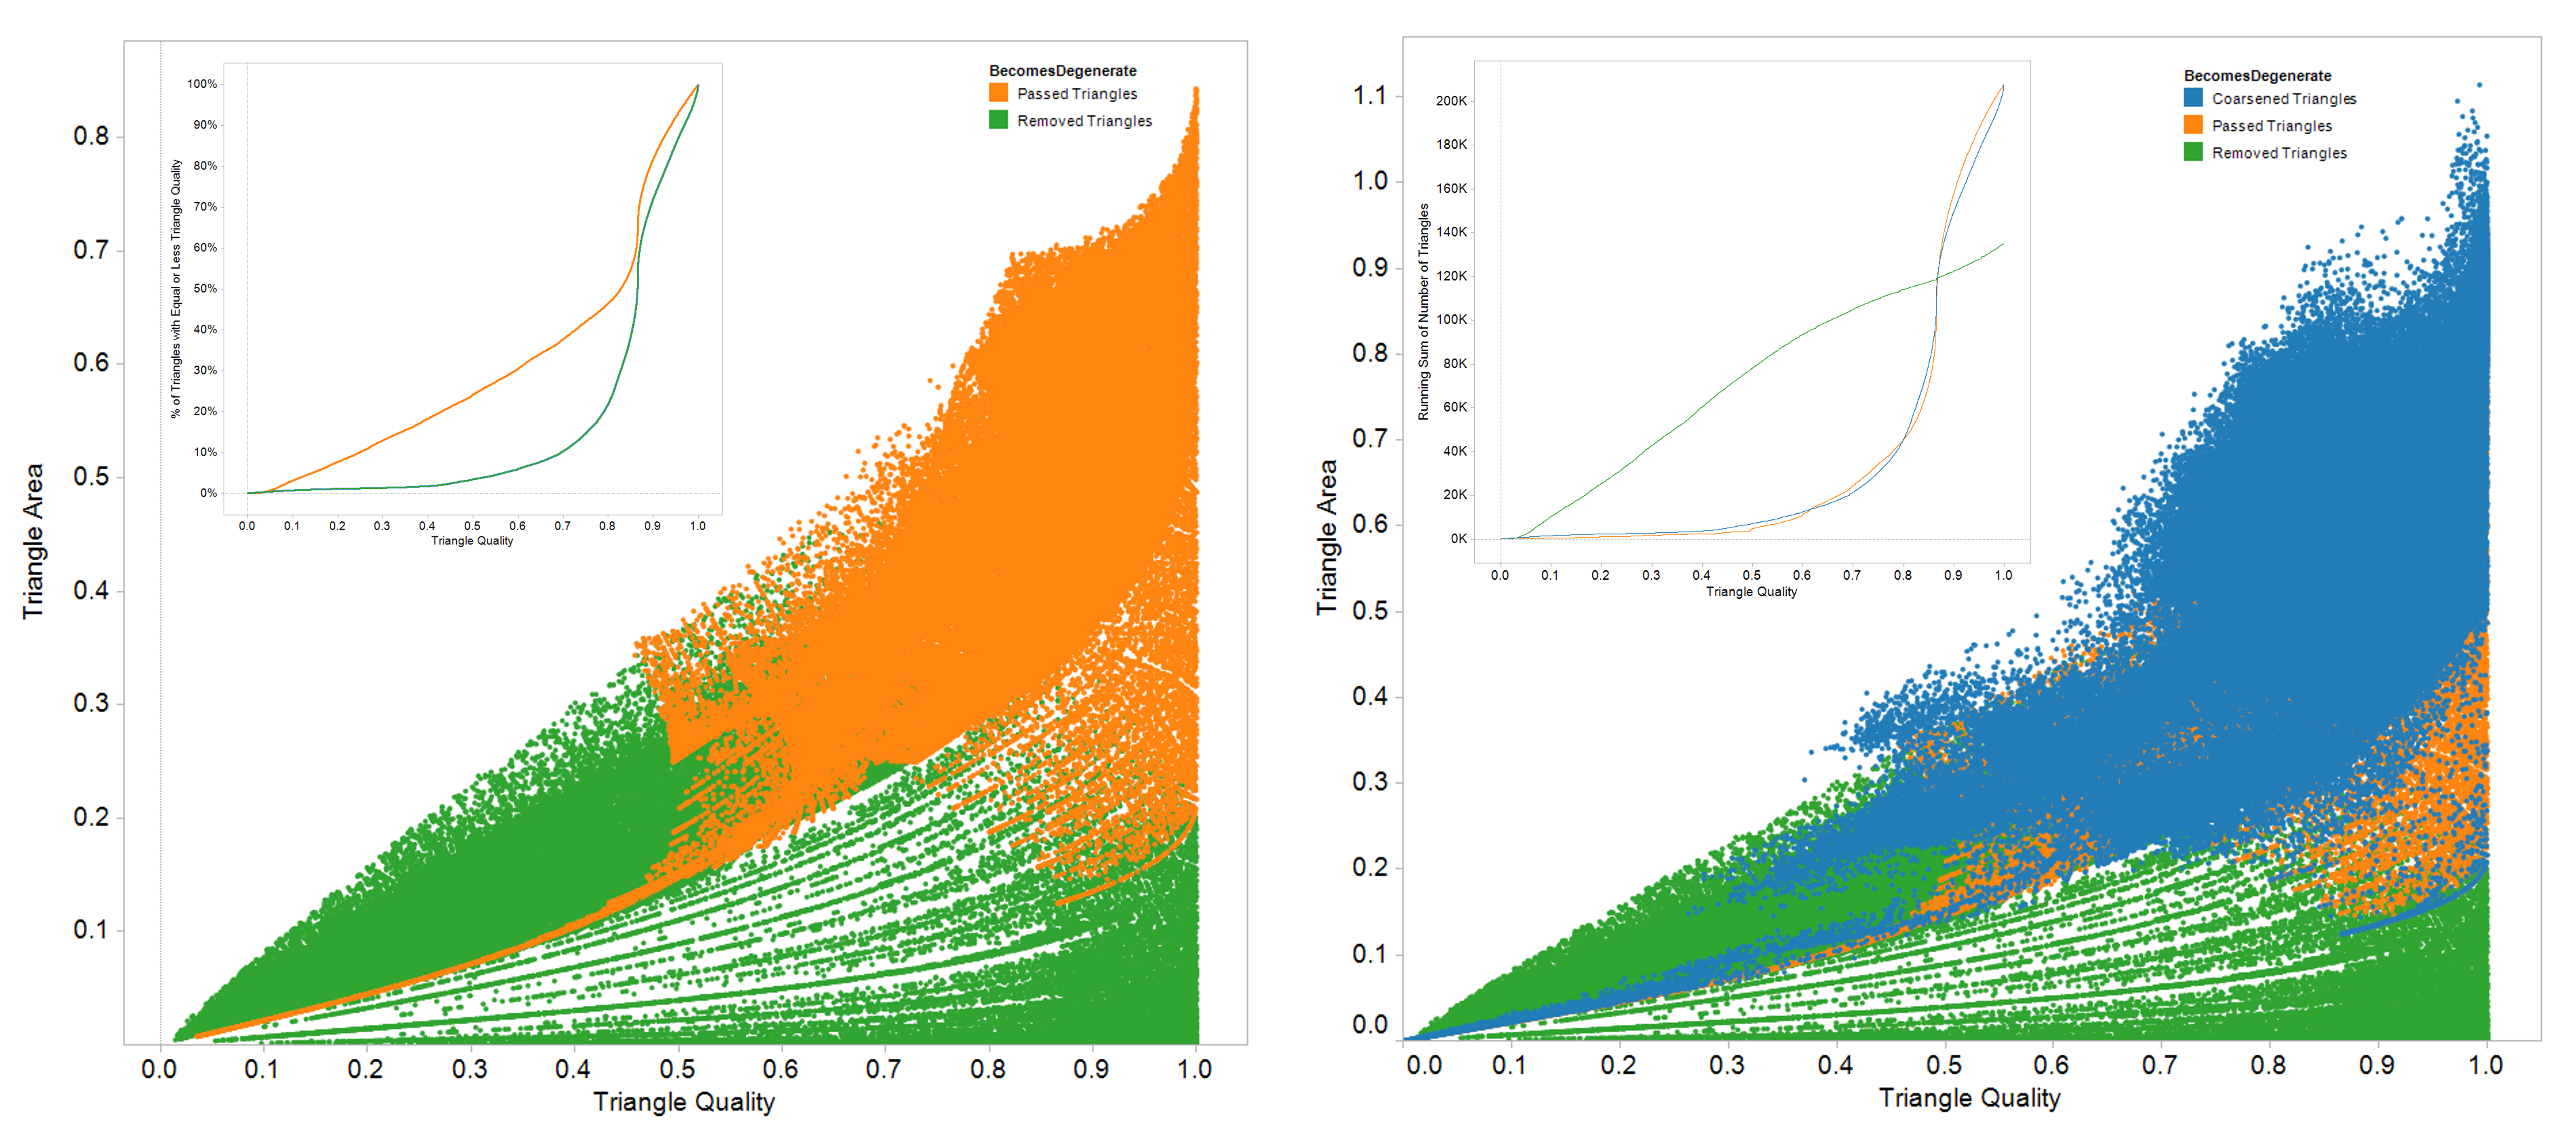
\includegraphics[width=\textwidth]{CoarseningGraphs}
\caption{Top left: Orange represents the triangles that the coarsening chose to keep. Green represents the triangles that the coarsening removed. Top right: Green and Orange are as in the top left. Blue represents the quality of the triangles that the orange triangles were modified into. Top left inset: distribution of triangle quality as compared between the original triangles, and the coarsened triangles. Top right inset: Distribution of triangle quality for coarsened, passed and removed triangles.}
\label{fig:coarseninggraphs}
\end{figure*}


Figure \ref{fig:coarsening} shows a before and after comparison of our coarsening technique with $k=1$. 
Figure \ref{fig:coarseninggraphs} shows the change in triangle quality before and after coarsening.

\subsubsection{Dual Mesh Generation}
To generate the dual of our triangular input meshes, we perform the following procedure: For each face, average the vertices to get the centroid, and store it in a new array at the same ID as the original face. Now the surrounding face lists for each of the vertices in the original mesh form a representation of each face of the dual mesh.

\subsubsection{Dual Mesh Generation Results}
Table~\ref{tab:timingsdualmesh} shows the timings for generating dual meshes.

\begin{table}[h!]
\begin{center}
\begin{tabular}{l r r r r r r r}
Architecture & V1 & V2 & V3 & V4 & V5 & V6 & V7\\
\hline
CUDA & 18 & 3 & $<1$ & $<1$ & 39 & 5 & $<1$ \\
OpenMP & ? & ? & ? & ? & ? & ? & ? \\
\end{tabular}
\caption{Timings for dual mesh generation}
\label{tab:timingsdualmesh}
\end{center}
\end{table}
\textcolor{red}{TODO: There's a bug in my dual mesh generation code that is giving me trouble. I need to fix it so I can make the figure and update the timings.}
\textcolor{red}{!!!!Figure!!!!} shows a mesh and its dual overlaid as a skeleton.

\section{Conclusions and Future Work}
We provide an efficient, generalized method for parallel generation of topological connectivity information. We require little to no alteration to the algorithms generating geometry, although small modifications to allow for knowledge of input topological features can be leveraged for better performance. We demonstrate how to use such modifications to gain performance on structured grids, and to perform a simple mesh coarsening on either structured or unstructured grids. We demonstrate that our algorithm is effective on structured grids and on several different tetrahedral grids. 

Future work includes measuring how this technique scales up approaching petascale and exascale and determining what bottlenecks, if any, need to be addressed for this transition. 
 
%% if specified like this the section will be ommitted in review mode
\acknowledgments{
This work was supported in full by the DOE Office of Science, Advanced Scientific Computing Research, under award number 10-014707, program manager Lucy Nowell.

Part of this work was performed by Sandia National Laboratories.  Sandia National Laboratories is a multi-program laboratory operated by Sandia Corporation, a wholly owned subsidiary of Lockheed Martin Corporation, for the U.S. Department of Energy's National Nuclear Security Administration.}

\bibliographystyle{abbrv}
%%use following if all content of bibtex file should be shown
\nocite{*}
\bibliography{template}
\end{document}